% !TEX TS-program = pdflatex
% !TEX encoding = UTF-8 Unicode

\documentclass[11pt]{article} % use larger type; default would be 10pt

\usepackage[utf8]{inputenc} % set input encoding (not needed with XeLaTeX)
\usepackage[T1]{fontenc} %font encoding ? --> need to clarify that

%%% PAGE DIMENSIONS
\usepackage{geometry} % to change the page dimensions
\geometry{a4paper} % or letterpaper (US) or a5paper or....
\geometry{margin=1in} % for example, change the margins to 2 inches all round

\usepackage{graphicx} % support the \includegraphics command and options
\usepackage[parfill]{parskip} % Activate to begin paragraphs with an empty line rather than an indent

%%% PACKAGES
\usepackage{listings}
\usepackage{polski}
\usepackage{amsmath}
\usepackage{amssymb}
\usepackage{booktabs} % for much better looking tables
\usepackage{array} % for better arrays (eg matrices) in maths
\usepackage{paralist} % very flexible & customisable lists (eg. enumerate/itemize, etc.)
\usepackage{verbatim} % adds environment for commenting out blocks of text & for better verbatim
\usepackage{subfig} % make it possible to include more than one captioned figure/table in a single float
% These packages are all incorporated in the memoir class to one degree or another...
\lstset{
  literate={ą}{{\k a}}1
  		     {Ą}{{\k A}}1
           {ż}{{\. z}}1
           {Ż}{{\. Z}}1
           {ź}{{\' z}}1
           {Ź}{{\' Z}}1
           {ć}{{\' c}}1
           {Ć}{{\' C}}1
           {ę}{{\k e}}1
           {Ę}{{\k E}}1
           {ó}{{\' o}}1
           {Ó}{{\' O}}1
           {ń}{{\' n}}1
           {Ń}{{\' N}}1
           {ś}{{\' s}}1
           {Ś}{{\' S}}1
           {ł}{{\l}}1
           {Ł}{{\L}}1
}
%%% HEADERS & FOOTERS
\usepackage{fancyhdr} % This should be set AFTER setting up the page geometry
\pagestyle{fancy} % options: empty , plain , fancy
\renewcommand{\headrulewidth}{0pt} % customise the layout...
\lhead{}\chead{}\rhead{}
\lfoot{}\cfoot{\thepage}\rfoot{}
%%% END Article customizations

%%% The "real" document content comes below...

\title{Usuń i wygraj - projekt AAL\\
\large Dokumentacja końcowa}
\author{Piotr Zmyślony, nr albumu 268833}
\date{} % Activate to display a given date or no date (if empty),
         % otherwise the current date is printed 

\begin{document}
\maketitle

\section{Opis problemu}
\subsection{Treść zadania}
Gra „Usuń i wygraj” polega na uzyskaniu jak największego wyniku przy sukcesywnym usuwaniu liczb z (ustalonej przed rozpoczęciem gry) listy liczb całkowitych \textsl{N}, dopóki nie pozostanie nam zbiór pusty. Operacja usunięcia liczby \textsl{N[i]} powoduje uzyskanie liczby punktów równej wybranej liczbie. Po usunięciu jednej liczby, wszystkie dwie sąsiednie (\textsl{N[i]-1} oraz \textsl{N[i]+1}) liczby, jeśli istnieją, również są usuwane - tym razem bez uzyskiwania jakichkolwiek punktów.

Problem polega na znalezieniu maksymalnej liczby punktów do zdobycia dla konkretnej listy.
\subsection{Analiza}
\subsubsection{Warianty listy}
Pierwszym krokiem jest posortowanie listy wstępnej rosnąco, co znacząco ułatwi dalszą analizę zagadnienia, stąd dalej przedstawione listy będą już posortowane.

Przypadkiem trywialnym problemu jest taka lista unikalnych liczb, w której  żadna z liczb nie posiada sąsiadów, na przykład \textsl{N1 = [-3,-1,1,3,5,7]}. W takim wypadku kolejność wyboru liczb nie ma znaczenia, ponieważ nigdy nie „tracimy” punktów poprzez usuwanie.

Przypadkiem ogólnym jest lista, w której liczby mogą posiadać sąsiadów,  na  przykład \textsl{N2 = [-10,-9,-8,1,2,3,4,5,7,8,9]}. Teraz musimy rozważać rozłączne, rosnące listy liczb sąsiadujących. Lista \textsl{N2} rozkłada się na listy: \textsl{[-10,-9,-8]}, \textsl{[1,2,3,4,5]}, \textsl{[7,8,9]}. Wynikiem jest suma maksymalnych ilości punktów, jaką można uzyskać w każdej z podlist.
\subsubsection{Problem duplikatów}
Problem duplikatów, czyli liczb występujących w liście po klika razy, można rozwiązać sumując wszystkie wystąpienia i zastępując je tą właśnie sumą. Na przykład dla \textsl{N3 = [1,1,2,3,3,3,4,4,4,6,7,7,8]} dostajemy: \textsl{[2,2,9,12]}, \textsl{[6,14,8]}.
Dla tych list, operacja usuwania zmienia się nieznacznie - usunięcie liczby \textsl{N[i]} powoduje usunięcie \textsl{N[i-1]} i \textsl{N[i+1]}.
\section{Algorytm}
\subsection{Przetwarzanie wstępne danych}
Na wstępie algorytm dostaje listę liczb całkowitych i tworzy rozłączne listy sąsiadujących i posortowanych rosnąco liczb. Na każdej z nich dokonywana jest operacja usuwania duplikatów opisana powyżej. Wynik sumaryczny właściwego algorytmu (opisanego poniżej) dla każdej z list jest odpowiedzią na to, jaki jest maksymalny możliwy do uzyskania wynik na liście początkowej.
\subsection{Działanie algorytmu}
Na początku algorytm dokonuje sprawdzenia, jakiego typu jest lista, czyli porównuje pierwszą (\textsl{min}) i ostatnią (\textsl{max}) liczbę w liście \textsl{N}
\begin{itemize}
  \item \textbf{Typ A} - \( min \geqslant 0\)
  \item \textbf{Typ B} - \( min < 0 \)	
\end{itemize}
\subsubsection{Rozwiązanie dla typu A}
Jest to najprostszy z przypadków, którego rozwiązanie ma złożoność \textsl{O(n)}. Służy do tego poniższy algorytm:
\begin{description}
\item[Algorytm House Robber:]\leavevmode
\begin{lstlisting}[language=Python]
def house_robber(array):
    incl = 0
    excl = 0

    for i in array:
        new_excl = excl if excl >= incl else incl
        incl = excl + i
        excl = new_excl
    return excl if excl > incl else incl
\end{lstlisting}
\end{description}
\subsubsection{Rozwiązanie dla typu B}
W tym wypadku algorytm powyższy (nawet z modyfikacjami) nie jest w stanie policzyć największej wartości.

W pierwszym kroku, sprawdzamy czy lista posiada również wartości większe bądź równe 0. Jeśli nie, wynik daje nam rekurencyjny \textsl{Algorytm I} opisany pokrótce poniżej. 

Jeżeli tak - część rozwiązania dla liczb nieujemnych możemy dostać poprzez algorytm \textsl{House Robber}. Istnieją 3 możliwe sposoby podziału takiej listy: usuwamy 0, usuwamy liczbę na lewo od 0, usuwamy liczbę na prawo od 0.
Dla każdego z tych podziałów część dodatnią rozwiązujemy algorytmem \textsl{House Robber}, a część ujemną \textsl{Algorytmem I}. Z tych 3 wyników wybieramy największy jako końcowy.\\

\begin{description}
\item[Algorytm I:]\leavevmode
\begin{lstlisting}
1. wynik := 0
2. Sprawdź które liczby mają maksymalny BU*.
3. Jeśli jest tylko jedna liczba M[i] o największym BU, 
   wynik += M[i], usuń M[i-1], M[i] i M[i+1] i przejdź do kroku 2.
4. Utwórz tablicę max[n], gdzie n to ilość liczb o maksymalnym BU.
5. Dla każdego i=0..(n-1) kolejno: 
 5.1. z := rezultat Algorytmu I dla listy bez M[i] i sąsiadów
 5.2. max[i] := wynik + M[i] + z.
6. wynik += maksymalna wartość z tablicy max[]
7. Zwróć wynik.

*Bilans Usunięcia dla liczby N[i] równy jest N[i]-N[i-1]-N[i+1].
\end{lstlisting}
\end{description}

\subsection{Testowanie}
\subsubsection{Złożoność obliczeniowa}
Złożoność algorytmu \textsl{House Robber} jest liniowa, wymaga jedynie sortowania w pre-processingu danych. Stąd dla samych liczb dodanich złożoność obliczeniowa wynosi \textsl{O(nlogn)}, co jest przedstawione na Rysunku \ref{rys1}.

Złożoność obliczeniowa \textsl{Algorytmu I} jest równa \textsl{O(n!)}, o ile jesteśmy w stanie wygenerwować taką listę, aby przy każdej rekurencji wszystkie liczby miały tą samą wartość \textsl{BU}. Taka lista jest prawdopodobnie niemożliwa do wygenerowania.

Ilość duplikatów w liście wstępnej ma znaczny wpływ na czas działania - przykładowo, jeżeli 50\% listy stanowią duplikaty, to efektywnie, nasze \textsl{n} jest mniejsze o 50\%.
Stąd, czym większa długość podlist utworzonych z listy wstępnej, tym znacznie większy czas obliczeń.

Na Rysunku 2 można zaobserwować wpływ \textsl{Algorytmu I} dla wartości bliskich 0 - gwałtowny wzrost czasu wykonania, aż do momentu, kiedy ilość liczb będzie większa od liczności zakresu z którego te liczby są generowane. Widać, że po tym wzroście, wpływ na kształt funkcji ma jedynie sortowanie liczb z listy początkowej. Dzieje się tak dlatego, że po sortowaniu i usunięciu duplikatów możemy otrzymać zbiór, który maksymalnie ma liczność taką samą jak zakres generacji - czas działania \textsl{Algorytmu I} jest z grubsza niezmienny.

\subsubsection{Testowanie dla ciągłych list}
Lista ciągła to lista wstępna, która po sortowaniu i usunięciu duplikatów daje tylko jedną, długą podlistę. Takie listy gwarantują, że część ujemnych liczb będzie liczona przez tylko jedno uruchomienie \textsl{Algorytmu I}, co pozwala lepiej zobrazować jego złożoność obliczeniową.

Wykres efektu testowania takich list jest przedstawiony na Rysunku 3. Możemy zaobserwować pojedyncze listy, dla których algorytm wykonywał się w czasie o kilka rzędów wielkości większym niż średnia. Są to przypadki, dla których \textsl{Algorytm I} często musi się rozgałęziać poprzez rekurencję, innymi słowy - częste są sytuacje, w których BU jest równe dla dużej ilości liczb pozostałych w liście.

Program potrafi generować takie listy po podaniu opcji -\textsl{-evil}.

Interesującym porównaniem jest Rysunek 4. Tutaj liczby generowane są losowo, z równym prawdopodobieństwem, więc ilość podlist również jest losowa. Porównując linię czerwoną i zieloną, możemy zaobserwować, że od pewnego momentu, czas wykonania dla mniejszego zakresu liczb zaczyna być większy (długość listy ok. 13000). Sugeruje to, że dla zakresu [-1000, 1000] zaczynają się generować bardzo długie ciągi liczb sąsiednich, przez co czas wykonania \textsl{Algorytmu I} znacznie wzrasta. Dla tej samej długości listy, ale zakresu [-3000, 3000], istnieje mniejsze prawdopodobieństwo utworzenia równie długich ciągów sąsiednich liczb. Jednak dla jeszcze większych długości listy (nie przedstawionych na Rysunku 4), zagęszczenie liczb z zakresu reprezentowanego przez czerwoną linię będzie wystarczająco duże, żeby często tworzyć ciągi sąsiadów dłuższe niż 1000 (maksymalny ciąg ujemnych sąsiadów dla zakresu [-1000, 1000]) i od tego momentu czas wykonania będzie z powrotem większy.


\begin{figure}[h]
\caption{Czas działania algorytmu dla list liczb dodanich}
\label{rys1}
\centering
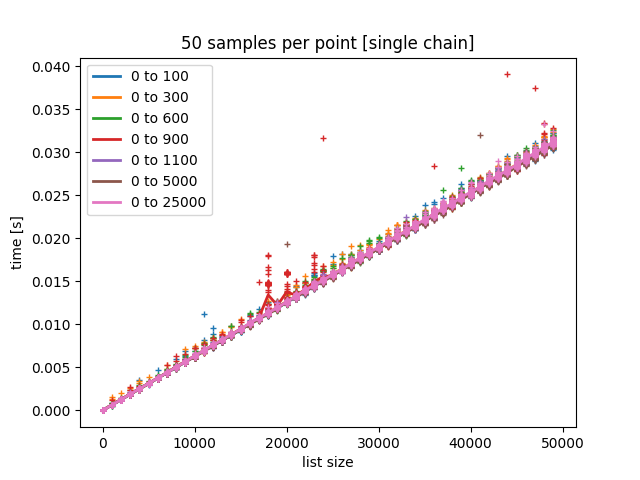
\includegraphics[scale=0.8]{50samples50000_0_25000}
\end{figure}

\begin{figure}[h]
\caption{Czas działania algorytmu dla list liczb ujemnych}
\label{rys2}
\centering
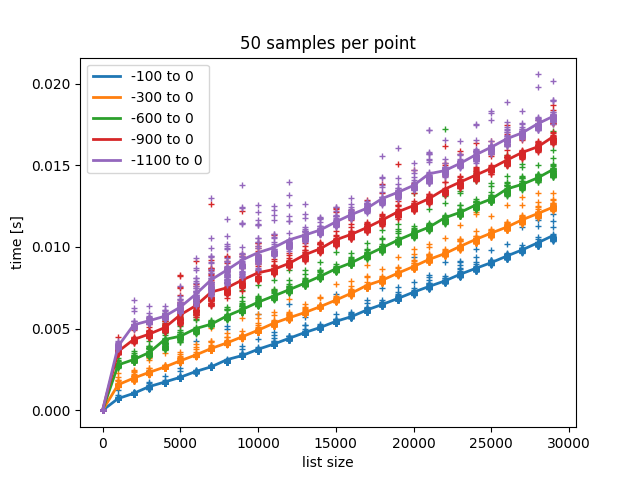
\includegraphics[scale=0.8]{50samples30000_-100_-1100}
\end{figure}

\begin{figure}[h]
\caption{Czas działania algorytmu dla listy, która zawiera tylko jedną, długą podlistę. Listy zaczynają się od -100, -1000 lub -10000}
\label{rys3}
\centering
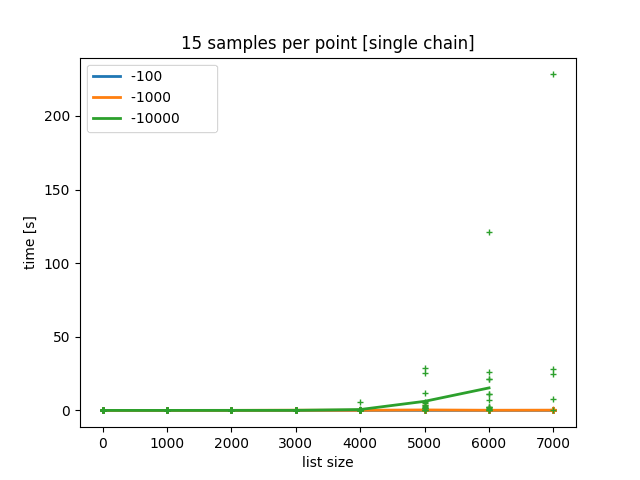
\includegraphics[scale=0.8]{bigboy}
\end{figure}

\begin{figure}[h]
\caption{Wpływ zagęszczenia i długich podlist na czas wykonania}
\label{rys4}
\centering
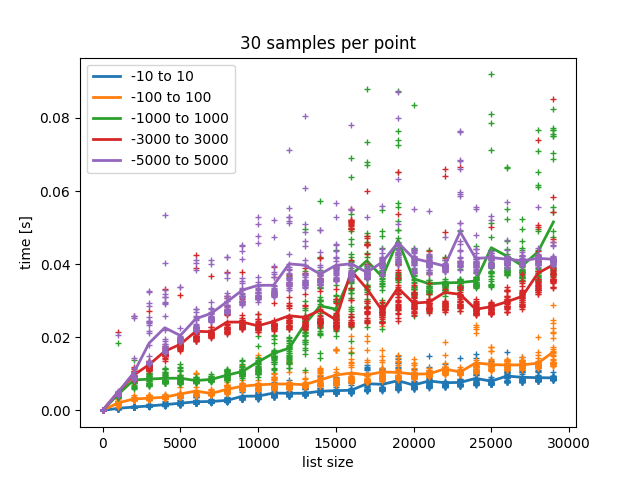
\includegraphics[scale=0.8]{sparsity}
\end{figure}

\subsubsection{Program}
Program potrafi działać w 4 trybach, definiowanych przez podanie opcji \textsl{-m <tryb>}.
\paragraph{Tryb 1} Odczytuje dane z stdin, każdą linię interpretując jako jedną instancję problemu (jedną listę liczb). Można go używać jako tryb interaktywny odczytujący dane z klawiatury lub wsadowy, jeśli dane mamy w pliku.
\paragraph{Tryb 2} Program sam generuje jedną instancję danych losowych o parametrach, takich jak np. zakres liczb, ilość liczb w liście.
\paragraph{Tryb 3} Program generuje dane losowe i testuje czasy działania algorytmu dla rosnącej ilości liczb w liście. Możliwe jest wyświetlenie wyniku działania na wykresie.
\paragraph{Tryb 4} Program przyjmuje na wejście pary liczb, które definiują zakres generacji liczb w liście wstępnej. Dla każdego zakresu wykonywany jest Tryb 3 programu, a końcowy wynik przedstawiany jest na wykresie. Tryb 4 najlepiej służy jako narzędzie do kompleksowego sprawdzania złożoności \textsl{Algorytmu I}.

Wszystkie atrybuty, które użytkownik może modyfikować są dostępne po podaniu opcji (\textsl{-\phantom{}-help} \textsl{python main.py -\phantom{}-help}).
\end{document}